% =============================================================================
% Double U-Net — Paper-style block diagram with project dimensions
% Paper: https://arxiv.org/abs/2006.04868
% Project: 3×384² input, 1×384² output
% =============================================================================
\documentclass[border=10pt]{standalone}
\usepackage[T1]{fontenc}
\usepackage{tikz}
\usepackage{xcolor}
\usepackage{amsmath}
\usetikzlibrary{arrows.meta, calc, fit, backgrounds, positioning}

% --- Colors matching the paper ---
\definecolor{vggyellow}{RGB}{255,200,50}
\definecolor{asppcyan}{RGB}{70,195,220}
\definecolor{dec1green}{RGB}{190,210,150}
\definecolor{enc2gold}{RGB}{255,210,100}
\definecolor{dec2green}{RGB}{155,210,160}
\definecolor{outred}{RGB}{170,25,25}
\definecolor{mulgreen}{RGB}{75,140,75}
\definecolor{netborder}{RGB}{0,155,215}
\definecolor{inputgray}{RGB}{245,245,245}

% --- Styles ---
\tikzset{
  sblk/.style={
    draw=black!50, semithick, fill=#1,
    minimum width=3.6cm, minimum height=0.55cm,
    font=\scriptsize\sffamily, inner sep=2pt, align=center,
  },
  wblk/.style={
    draw=black!55, semithick, fill=#1,
    minimum width=3.6cm, minimum height=0.6cm,
    font=\scriptsize\sffamily\bfseries, inner sep=2pt, align=center,
  },
  vblk/.style={
    draw=black!55, semithick, fill=vggyellow,
    minimum width=3.6cm, minimum height=2.4cm,
    font=\footnotesize\sffamily\bfseries, inner sep=4pt, align=center,
  },
  flowarr/.style={-{Stealth[length=4pt]}, thick, black!65},
  skiparr/.style={-{Stealth[length=3.5pt]}, semithick, black!50, densely dash dot},
}

% --- Layout constants ---
\def\bw{3.6}       % block width cm
\def\Lx{0}         % Net1 center x
\def\Rx{6.5}       % Net2 center x
\def\sg{0.02}      % stack gap between blocks

\begin{document}
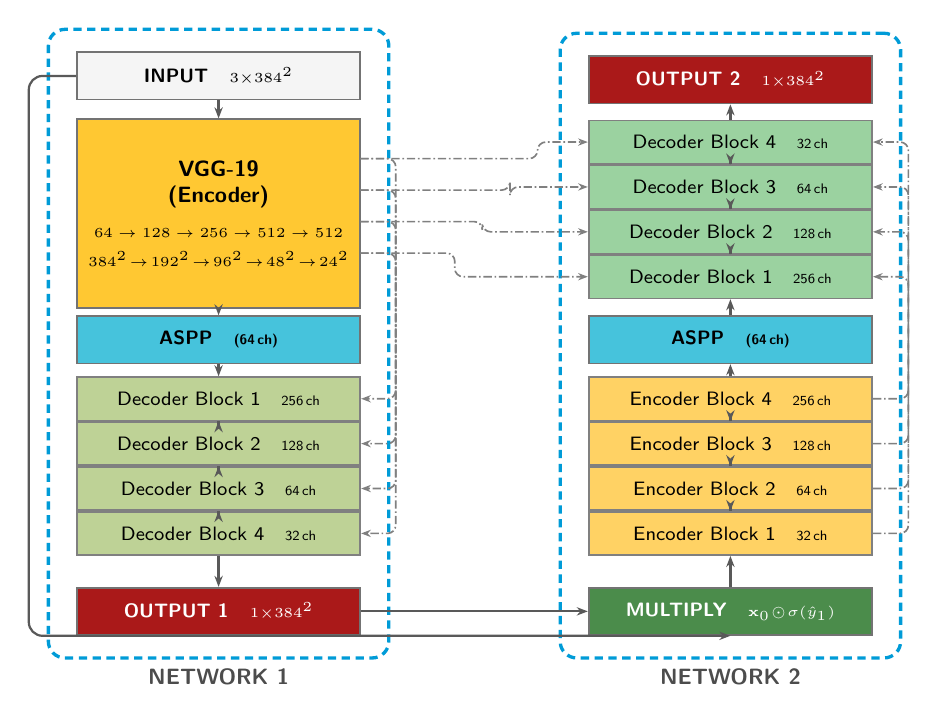
\begin{tikzpicture}[y=-1cm]

% =====================================================================
%  NETWORK 1
% =====================================================================

% INPUT — dimension inside the block
\node[wblk=inputgray] (inp) at (\Lx, 0) {INPUT\quad{\tiny$3{\times}384^2$}};

% VGG-19 Encoder — all info inside
\node[vblk] (vgg) at (\Lx, 1.75) {%
  VGG-19\\(Encoder)\\[3pt]
  {\tiny\normalfont 64\;$\to$\;128\;$\to$\;256\;$\to$\;512\;$\to$\;512}\\[1pt]
  {\tiny\normalfont $384^2\!\to\!192^2\!\to\!96^2\!\to\!48^2\!\to\!24^2$}};

% ASPP 1
\node[wblk=asppcyan] (aspp1) at (\Lx, 3.35) {ASPP\quad{\tiny(64\,ch)}};

% Decoder 1 — channel counts inside blocks
\node[sblk=dec1green] (d1b1) at (\Lx, 4.1) {Decoder Block 1\quad{\tiny 256\,ch}};
\node[sblk=dec1green] (d1b2) at (\Lx, 4.1 + 0.55 + \sg) {Decoder Block 2\quad{\tiny 128\,ch}};
\node[sblk=dec1green] (d1b3) at (\Lx, 4.1 + 2*0.55 + 2*\sg) {Decoder Block 3\quad{\tiny 64\,ch}};
\node[sblk=dec1green] (d1b4) at (\Lx, 4.1 + 3*0.55 + 3*\sg) {Decoder Block 4\quad{\tiny 32\,ch}};

% OUTPUT 1 — dimension inside the block
\node[wblk=outred, text=white] (out1) at (\Lx, 6.8) {OUTPUT 1\quad{\tiny$1{\times}384^2$}};

% --- Flow arrows Net1 ---
\draw[flowarr] (inp) -- (vgg);
\draw[flowarr] (vgg) -- (aspp1);
\draw[flowarr] (aspp1) -- (d1b1);
\draw[flowarr] (d1b1) -- (d1b2);
\draw[flowarr] (d1b2) -- (d1b3);
\draw[flowarr] (d1b3) -- (d1b4);
\draw[flowarr] (d1b4) -- (out1);

% --- Skip connections VGG → Decoder 1 ---
\foreach \decnode/\vy in {d1b1/1.05, d1b2/1.45, d1b3/1.85, d1b4/2.25} {
  \draw[skiparr, rounded corners=3pt]
    (\Lx + \bw/2, \vy) -- ++(0.45, 0) |- (\decnode.east);
}

% =====================================================================
%  NETWORK 2  (flow goes UPWARD)
% =====================================================================

% MULTIPLY
\node[wblk=mulgreen, text=white] (mul) at (\Rx, 6.8)
  {MULTIPLY\quad{\tiny$\mathbf{x}_0 \!\odot\! \sigma(\hat{y}_1)$}};

% Encoder 2 — channel counts inside blocks
\node[sblk=enc2gold] (e2b1) at (\Rx, 4.1 + 3*0.55 + 3*\sg) {Encoder Block 1\quad{\tiny 32\,ch}};
\node[sblk=enc2gold] (e2b2) at (\Rx, 4.1 + 2*0.55 + 2*\sg) {Encoder Block 2\quad{\tiny 64\,ch}};
\node[sblk=enc2gold] (e2b3) at (\Rx, 4.1 + 0.55 + \sg) {Encoder Block 3\quad{\tiny 128\,ch}};
\node[sblk=enc2gold] (e2b4) at (\Rx, 4.1) {Encoder Block 4\quad{\tiny 256\,ch}};

% ASPP 2
\node[wblk=asppcyan] (aspp2) at (\Rx, 3.35) {ASPP\quad{\tiny(64\,ch)}};

% Decoder 2 — channel counts inside blocks
\node[sblk=dec2green] (d2b1) at (\Rx, 2.55) {Decoder Block 1\quad{\tiny 256\,ch}};
\node[sblk=dec2green] (d2b2) at (\Rx, 1.98) {Decoder Block 2\quad{\tiny 128\,ch}};
\node[sblk=dec2green] (d2b3) at (\Rx, 1.41) {Decoder Block 3\quad{\tiny 64\,ch}};
\node[sblk=dec2green] (d2b4) at (\Rx, 0.84) {Decoder Block 4\quad{\tiny 32\,ch}};

% OUTPUT 2
\node[wblk=outred, text=white] (out2) at (\Rx, 0.05) {OUTPUT 2\quad{\tiny$1{\times}384^2$}};

% --- Flow arrows Net2 (upward) ---
\draw[flowarr] (mul) -- (e2b1);
\draw[flowarr] (e2b1) -- (e2b2);
\draw[flowarr] (e2b2) -- (e2b3);
\draw[flowarr] (e2b3) -- (e2b4);
\draw[flowarr] (e2b4) -- (aspp2);
\draw[flowarr] (aspp2) -- (d2b1);
\draw[flowarr] (d2b1) -- (d2b2);
\draw[flowarr] (d2b2) -- (d2b3);
\draw[flowarr] (d2b3) -- (d2b4);
\draw[flowarr] (d2b4) -- (out2);

% --- Skip connections Encoder 2 → Decoder 2 (right side) ---
\foreach \enc/\dec in {e2b4/d2b1, e2b3/d2b2, e2b2/d2b3, e2b1/d2b4} {
  \draw[skiparr, rounded corners=3pt]
    (\enc.east) -- ++(0.45, 0) |- (\dec.east);
}

% =====================================================================
%  CROSS-NETWORK CONNECTIONS
% =====================================================================

% OUTPUT 1 → MULTIPLY (horizontal)
\draw[flowarr] (out1) -- (mul);

% INPUT → MULTIPLY (route along left edge then across bottom)
\draw[flowarr, rounded corners=5pt]
  (inp.west) -- ++(-0.6, 0) |- (mul.south);

% VGG → Decoder 2 cross-skip (through gap between networks)
\draw[skiparr, rounded corners=3pt]
  (\Lx + \bw/2, 1.05) -- ++(2.25, 0) |- (d2b4.west);
\draw[skiparr, rounded corners=3pt]
  (\Lx + \bw/2, 1.45) -- ++(1.9, 0) |- (d2b3.west);
\draw[skiparr, rounded corners=3pt]
  (\Lx + \bw/2, 1.85) -- ++(1.55, 0) |- (d2b2.west);
\draw[skiparr, rounded corners=3pt]
  (\Lx + \bw/2, 2.25) -- ++(1.2, 0) |- (d2b1.west);

% =====================================================================
%  NETWORK BORDERS (dashed cyan)
% =====================================================================
\begin{scope}[on background layer]
  \node[draw=netborder, very thick, densely dashed,
        rounded corners=6pt,
        fit=(inp)(vgg)(aspp1)(d1b4)(out1),
        inner xsep=10pt, inner ysep=8pt] (n1box) {};

  \node[draw=netborder, very thick, densely dashed,
        rounded corners=6pt,
        fit=(out2)(d2b4)(aspp2)(e2b4)(e2b1)(mul),
        inner xsep=10pt, inner ysep=8pt] (n2box) {};
\end{scope}

% Network labels
\node[font=\footnotesize\sffamily\bfseries, text=black!70,
      anchor=north] at (n1box.south) {NETWORK 1};
\node[font=\footnotesize\sffamily\bfseries, text=black!70,
      anchor=north] at (n2box.south) {NETWORK 2};

\end{tikzpicture}
\end{document}
